\FloatBarrier
\section{Kernel-Independent Fast Multipole Method}\label{sec:KIFMM}
\sectionmark{KIFMM}

The KIFMM method retains the same structure as the original FMM algorithms but changes the way in which the potentials are represented and how the expansions and translations are computed. In order to remove the need to expand the kernel using multipole expansions, an alternative method of accurately representing all particles in a node is required which requires fewer operations than the number of particles in the node. Ying \cite{Ying2004} proposes the use of equivalent surfaces which can capture the effect of the potential inside a node. We can then translate these surface potentials using only kernel evaluations and then evaluate the effect of these surfaces on the particle position.

In order to explain how the KIFMM method is adapted from the original FMM algorithm, we will first explain how the KIFMM decomposes the domain. The main difference is the use of multiple interaction lists to evaluate the potential of different nodes. 

\subsection{Hierarchical decomposition}
Let $\mathcal{D}$ be the computational domain, which is defined to be a cube in $\mathcal{R}^3$ such that it encompasses all points in $\{\bm{y}_n\}$ and $\{\bm{x}_m\}$. This is typically defined to be the smallest possible cube which includes all the points. The KIFMM method in three dimensions builds an Octree structure of cubes in 3D with the cube $\mathcal{D}$ as the root node. This node will be labelled the Level $0$ partition where no subdivision has occurred. Each subsequent division is made of $8$ equal-sized cubes each with a side length of half of the cube above. For each level, every node is subdivided into $8$ children when the number of source points or target points within the cube is greater than some threshold $s\geq 1$. For efficiency, only points of the type which exceed the threshold are moved to the child nodes. This subdivision creates a new level $L+1$ containing the children of all subdivided nodes in level $L$. The node on level $L$ is referred to as the parent of nodes on level $L+1$. This process is repeated until all cubes have less than $s$ source or target points contained within them which is referred to as leaf nodes.

An example of a simple decomposition can be seen in \cref{fig:Decompostionexample}. In the non-adaptive case, if any node has greater than $s$ source points, then all nodes on that level are subdivided creating $8^L$ new nodes. We might choose to implement a tree of this form when the potential distribution is uniform as it reduces the types and complexity of the interactions described later, but we will only consider the adaptive case in this discussion as it is more efficient in the non-uniform cases we will be considering.

\subsubsection{Interaction Lists}
For any node $B$ in the Octree, its relation to its neighbouring nodes is defined through 4 interaction lists $I_U^B, I_V^B, I_X^B$ and $I_W^B$.

\begin{itemize}
\item The list $I^B_U$ contains $B$ itself and all leaf nodes which are adjacent to $B$. The $U$ list is empty for any non-leaf nodes.

\item The list $I_V^B$ contains all nodes which are children of the nodes which are neighbours of $B$'s parent. This means all nodes in $I_U^B$ are of the same level as B.

\item If $B$ is a leaf node then the interaction list $I_W^B$ contains all descendants of $B$'s neighbours whose parents are adjacent to $B$ but are not adjacent to $B$ themselves. In order to avoid computing the effect of the node twice, only nodes $A$, where $A$ and all its decedents, obey the conditions above are included. If $B$ is not a leaf node then $I_W^B$ is empty.

\item The list $I_X^B$ contains all nodes $A$ in which $B$ appears in the interaction list $I_W^A$.
\end{itemize}

\begin{figure}
    \centering
    \resizebox{.5\linewidth}{!}{\begin{tikzpicture}
    \node[anchor = south west,inner sep=0] (image) at (0,0) {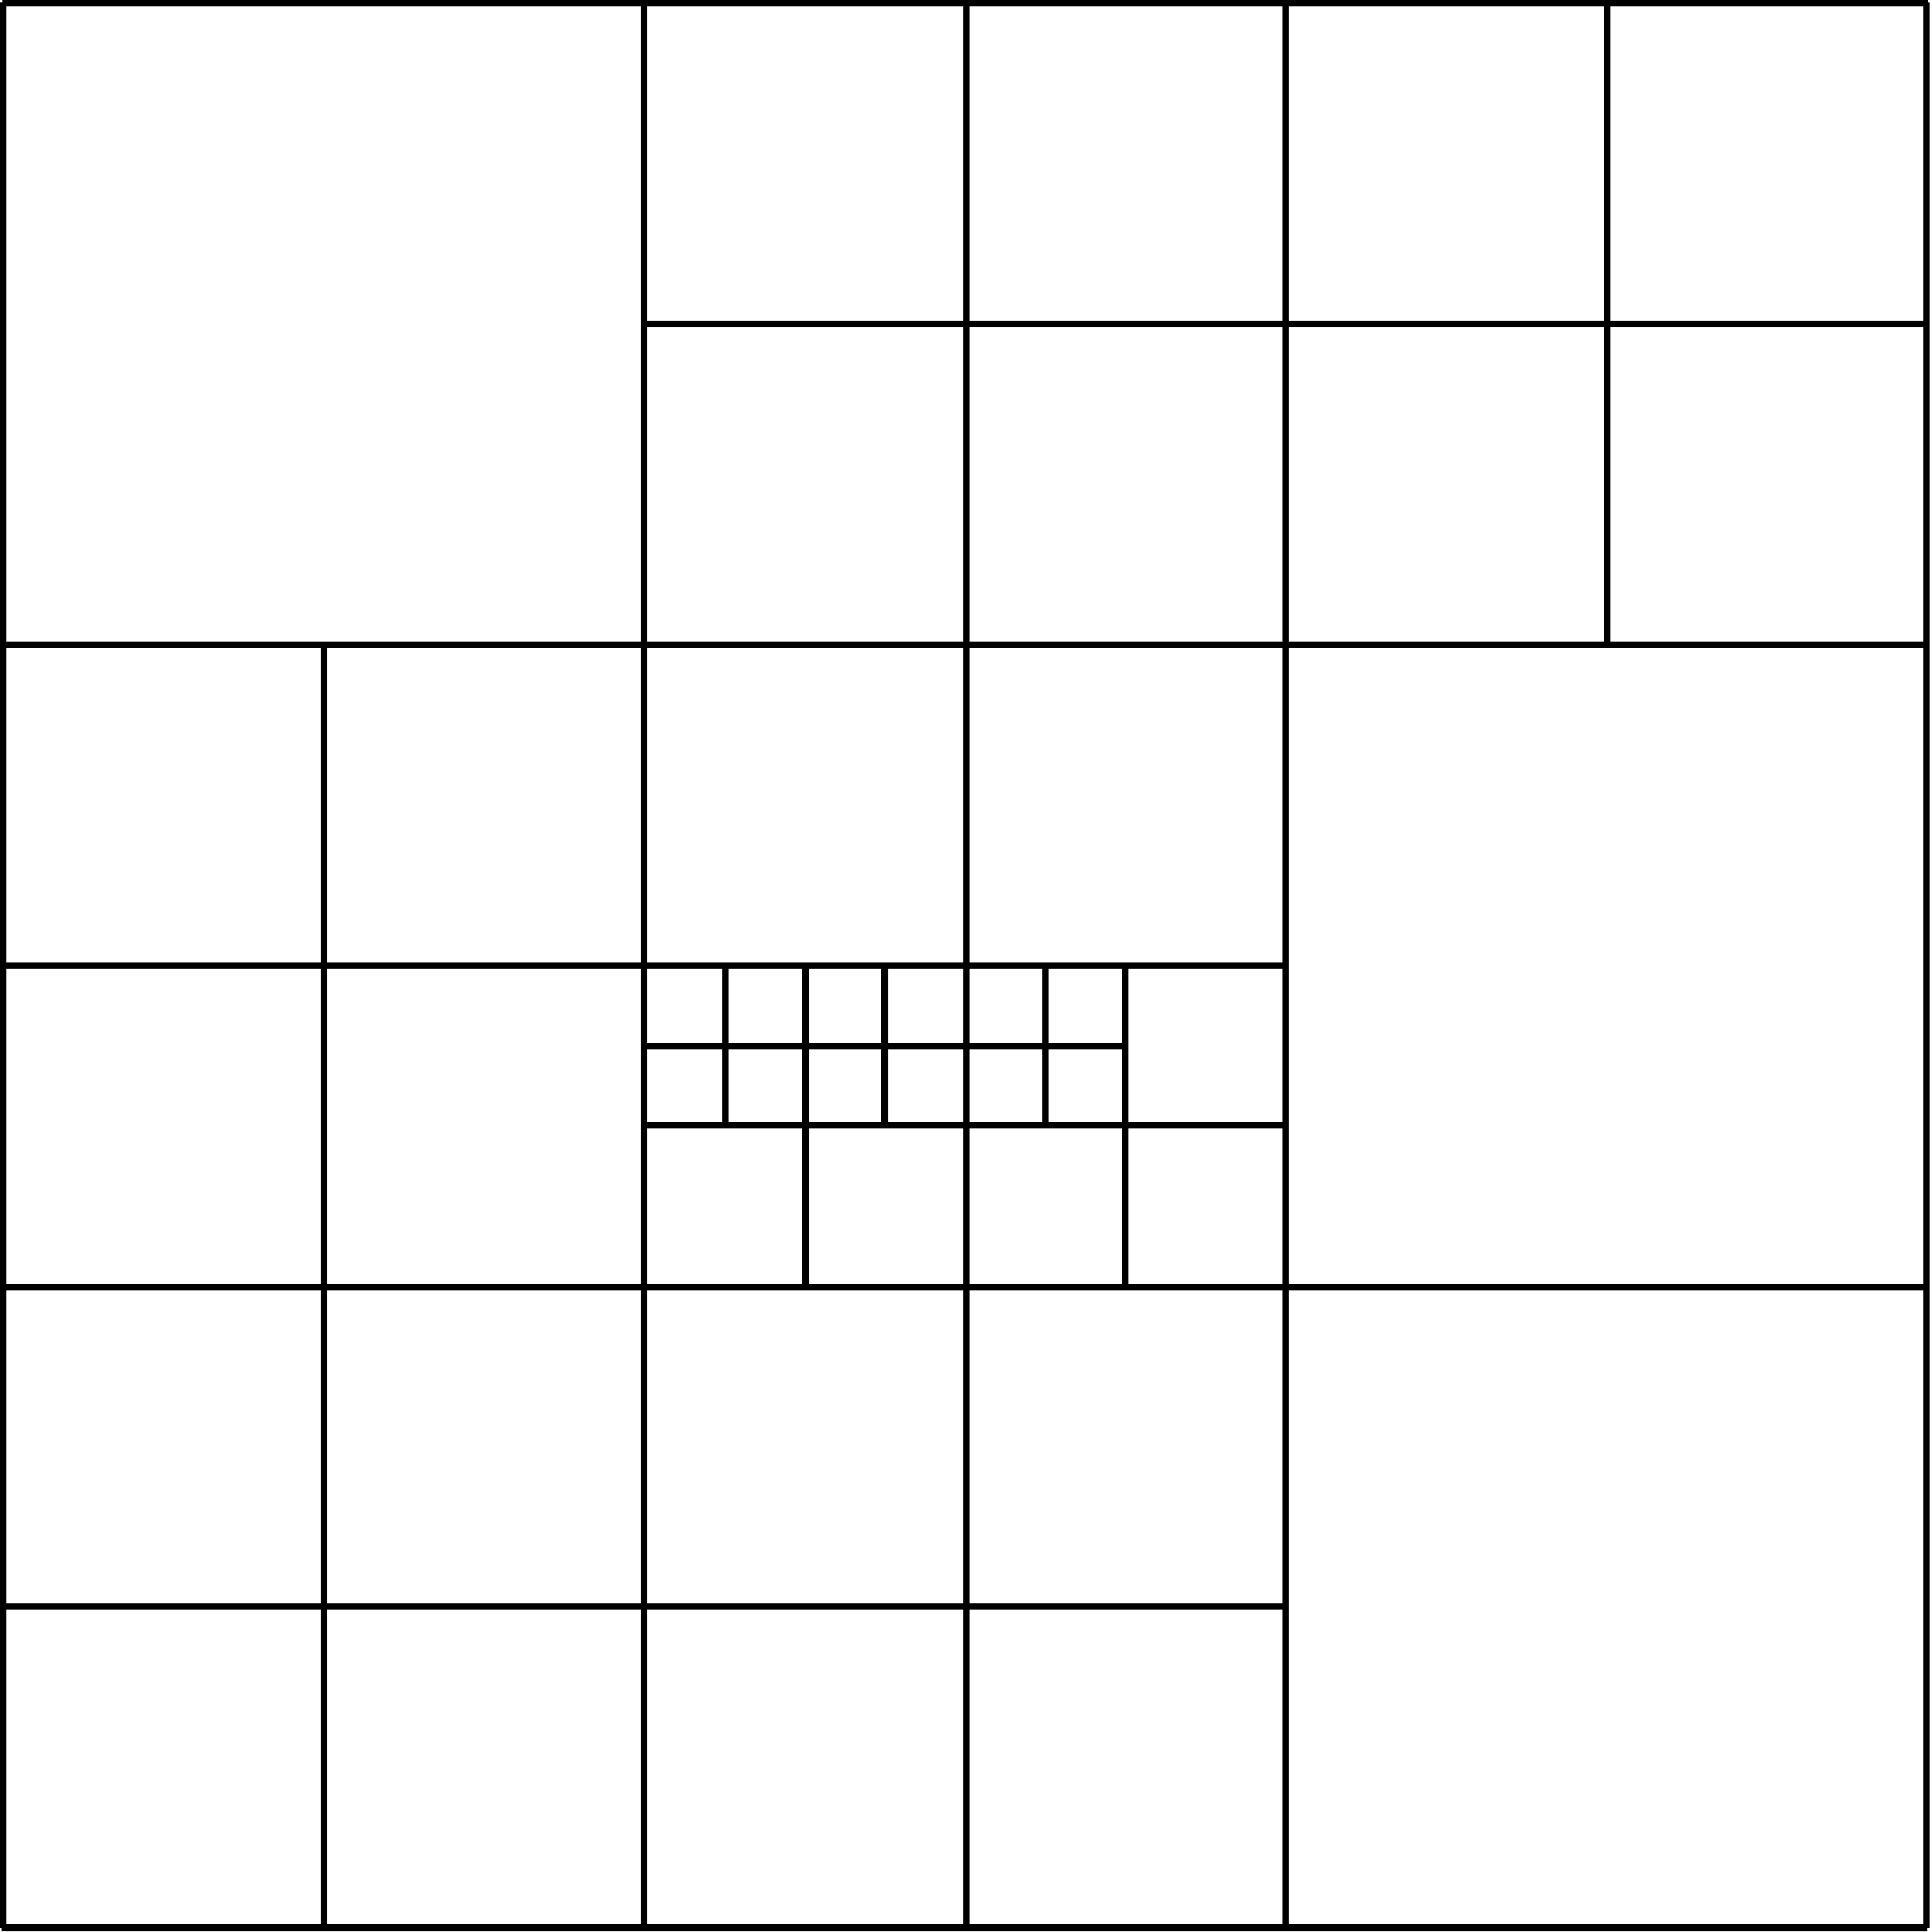
\includegraphics[width=.6\textwidth]{Images/KIFMM/Interaction.pdf}};
    \begin{scope}[x={(image.south east)},y={(image.north west)}]
    \begin{scope}[x={(image.south east)},y={(image.north west)}]
        \node at (0.165,0.83) {U};
        \node at (0.42,0.915) {V};
        \node at (0.58,0.915) {V};
        \node at (0.75,0.915) {V};
        \node at (0.91,0.915) {V};
        \node at (0.42,0.75) {U};
        \node at (0.58,0.75) {U};
        \node at (0.75,0.75) {V};
        \node at (0.91,0.75) {V};
        \node at (0.08,0.58) {V};
        \node at (0.25,0.58) {U};
        \node at (0.42,0.58) {{\color{red} \underline{B}}};
        \node at (0.58,0.58) {U};
        \node at (0.83,0.5) {X};
        \node at (0.08,0.42) {V};
        \node at (0.25,0.42) {U};
        \node at (0.355,0.48) {\tiny U};
        \node at (0.40,0.48) {\tiny U};
        \node at (0.44,0.48) {\tiny U};
        \node at (0.48,0.48) {\tiny U};
        \node at (0.52,0.48) {\tiny U};
        \node at (0.56,0.48) {\tiny W};
        \node at (0.62,0.46) {W};
        \node at (0.355,0.44) {\tiny W};
        \node at (0.40,0.44) {\tiny W};
        \node at (0.44,0.44) {\tiny W};
        \node at (0.48,0.44) {\tiny W};
        \node at (0.52,0.44) {\tiny W};
        \node at (0.56,0.44) {\tiny W};
        \node at (0.38,0.38) {W};
        \node at (0.46,0.38) {W};
        \node at (0.54,0.38) {W};
        \node at (0.62,0.38) {W};
        \node at (0.08,0.25) {V};
        \node at (0.25,0.25) {V};
        \node at (0.42,0.25) {V};
        \node at (0.58,0.25) {V};
        \node at (0.83,0.16) {X};
        \node at (0.08,0.08) {V};
        \node at (0.25,0.08) {V};
        \node at (0.42,0.08) {V};
        \node at (0.58,0.08) {V};
    \end{scope}
    \end{scope}
\end{tikzpicture}
}
    \caption{A 2D example of the interaction lists $I_U^B, I_V^B, I_X^B$ and $I_W^B$ for a node $B$}
    \label{fig:InteractionsLists}
\end{figure}


In figure\ref{fig:InteractionsLists} we show the 2D interaction lists for a node $B$ for a random arrangement of nodes, note that these might not all be leaf nodes. The interaction list for a node contains all the nodes that need to be considered through translations as well as the node's parent which transmits information about potential further out. These interactions can be grouped into two groups, the near and far-field interactions. Near field nodes are all nodes in $I_U^B$ and $I_X^B$ and will be denoted by $\mathcal{N}(B)$. The far-field contains all remaining nodes. While geometrically these definitions may be convoluted in the adaptive case, with nodes in the far-field being geometrically closer than those in the near field, they provide definitions for which nodes need to be computed directly or through the use of equivalent surfaces.

\subsection{Equivalent surfaces}

The KIFMM makes use of two equivalent surfaces for each node in the Octree to approximate the effect between source and source points inside and outside the node. The upwards equivalent surface is taken to be the boundary of the node $B$ (denoted $\Omega^U$) and the downwards equivalent surface to be the surface of a cube of width three times larger and centred on the node $B$ (denoted $\Omega^D$) as illustrated in \cref{fig:UpandDownsurf} \cite{Ying2004}. Upon both of these surfaces, equivalent potential densities $\bm{f}^{BU}$ and $\bm{f}^{BD}$ are denoted for the upwards and downwards equivalent surfaces of a node $B$ respectively. The upward equivalent surface is used to approximate the effect of all source points contained within the node and its decedents \cite{Rostami2016Kernel-independentStokeslets,Yan}. As such every point $\bm{x}\in\mathcal{F}(B)$ the velocity induced by that of the equivalent surface is the same as that induced by all source points in $B$, this gives that
\begin{equation}
\label{eq:upsurfint}
    \forall \;\bm{x} \in \mathcal{F}(B): \quad \int_{\Omega^U} S^\epsilon(\bm{x}, \bm{y}) \bm{f}^{BU}(\bm{y}) d \bm{y}=\sum_{{\bm{y}}_n \in B} S^\epsilon\left(\bm{x}, {\bm{y}}_n\right) {\bm{f}}_{n}
\end{equation}

The same can be applied to the downwards equivalent surface where instead, the contributions are obtained from source points in $\mathcal{F}(B)$. For any point in $B$ the velocity induced by the downwards surface equals that induced by the source points in $\mathcal{F}(B)$, which again gives
\begin{equation}
\label{eq:downsurfint}
    \forall \;\bm{x} \in B: \quad \int_{\Omega^D} S^\epsilon(\bm{x}, \bm{y}) \bm{f}^{BD}(\bm{y}) d \bm{y}=\sum_{{\bm{y}}_n \in \mathcal{F}(B)} S^\epsilon\left(\bm{x}, {\bm{y}}_n\right) {\bm{f}}_{n}
\end{equation}

\begin{figure}[ht]
    \centering
    \resizebox{.6\linewidth}{!}{% This file was created by matlab2tikz.
%
%The latest updates can be retrieved from
%  http://www.mathworks.com/matlabcentral/fileexchange/22022-matlab2tikz-matlab2tikz
%where you can also make suggestions and rate matlab2tikz.
%
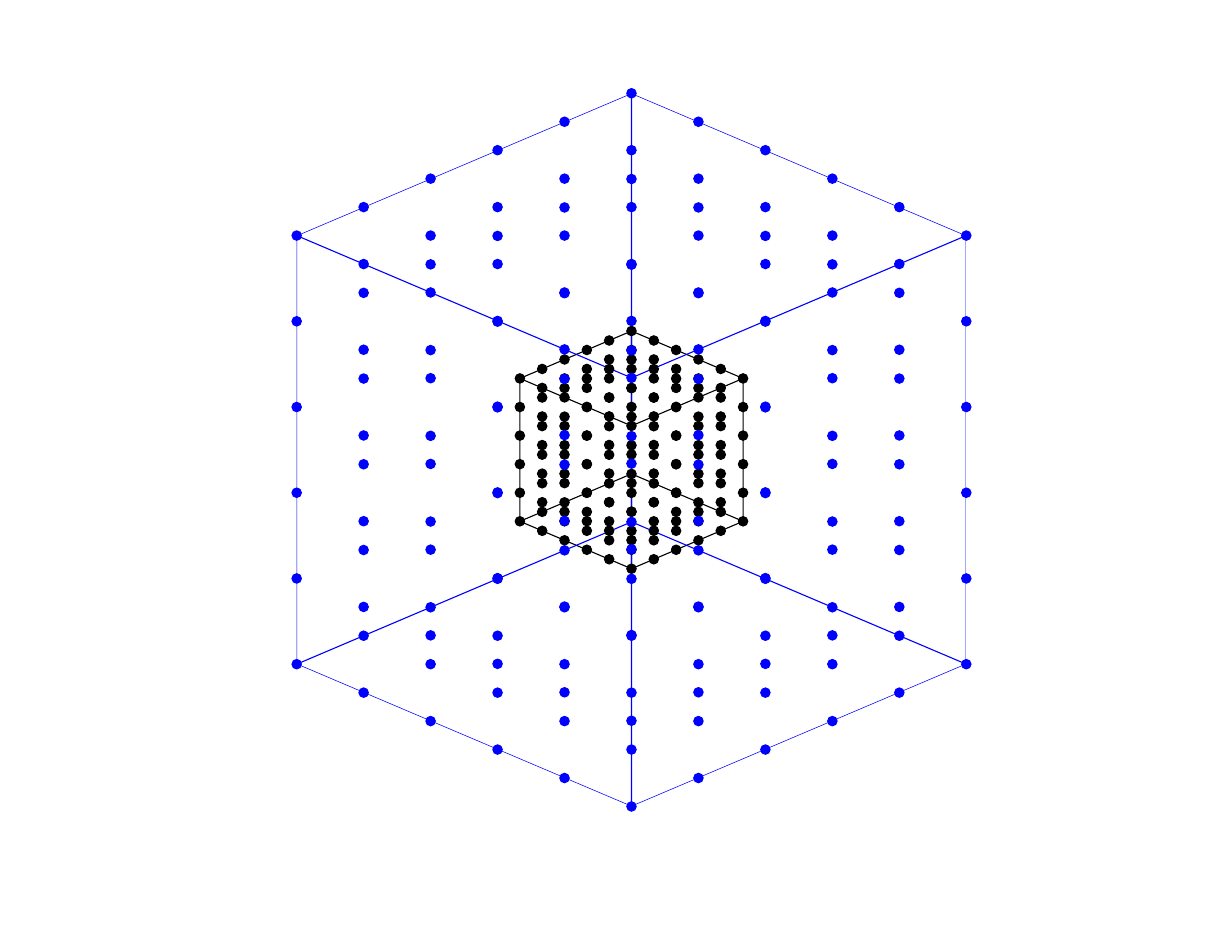
\begin{tikzpicture}

\begin{axis}[%
width=3.348in,
height=3.566in,
at={(1.345in,0.481in)},
scale only axis,
plot box ratio=1 1 1,
unbounded coords=jump,
xmin=-0.793615595547456,
xmax=1.67889551819639,
tick align=outside,
ymin=-0.793615595547456,
ymax=1.67889551819639,
zmin=-0.793615595547456,
zmax=1.67889551819639,
view={45}{25.15},
axis line style={draw=none},
ticks=none,
axis x line*=bottom,
axis y line*=left,
axis z line*=left
]
\addplot3 [color=black, only marks, mark size=1.7pt, mark=*, mark options={solid, black}]
 table[row sep=crcr] {%
0.0305547757004935	0.0305547757004935	0.0305547757004935\\
0.0305547757004935	0.195388849950083	0.0305547757004935\\
0.0305547757004935	0.360222924199673	0.0305547757004935\\
0.0305547757004935	0.525056998449263	0.0305547757004935\\
0.0305547757004935	0.689891072698853	0.0305547757004935\\
0.0305547757004935	0.854725146948443	0.0305547757004935\\
0.195388849950083	0.0305547757004935	0.0305547757004935\\
0.195388849950083	0.195388849950083	0.0305547757004935\\
0.195388849950083	0.360222924199673	0.0305547757004935\\
0.195388849950083	0.525056998449263	0.0305547757004935\\
0.195388849950083	0.689891072698853	0.0305547757004935\\
0.195388849950083	0.854725146948443	0.0305547757004935\\
0.360222924199673	0.0305547757004935	0.0305547757004935\\
0.360222924199673	0.195388849950083	0.0305547757004935\\
0.360222924199673	0.360222924199673	0.0305547757004935\\
0.360222924199673	0.525056998449263	0.0305547757004935\\
0.360222924199673	0.689891072698853	0.0305547757004935\\
0.360222924199673	0.854725146948443	0.0305547757004935\\
0.525056998449263	0.0305547757004935	0.0305547757004935\\
0.525056998449263	0.195388849950083	0.0305547757004935\\
0.525056998449263	0.360222924199673	0.0305547757004935\\
0.525056998449263	0.525056998449263	0.0305547757004935\\
0.525056998449263	0.689891072698853	0.0305547757004935\\
0.525056998449263	0.854725146948443	0.0305547757004935\\
0.689891072698853	0.0305547757004935	0.0305547757004935\\
0.689891072698853	0.195388849950083	0.0305547757004935\\
0.689891072698853	0.360222924199673	0.0305547757004935\\
0.689891072698853	0.525056998449263	0.0305547757004935\\
0.689891072698853	0.689891072698853	0.0305547757004935\\
0.689891072698853	0.854725146948443	0.0305547757004935\\
0.854725146948443	0.0305547757004935	0.0305547757004935\\
0.854725146948443	0.195388849950083	0.0305547757004935\\
0.854725146948443	0.360222924199673	0.0305547757004935\\
0.854725146948443	0.525056998449263	0.0305547757004935\\
0.854725146948443	0.689891072698853	0.0305547757004935\\
0.854725146948443	0.854725146948443	0.0305547757004935\\
0.0305547757004935	0.0305547757004935	0.195388849950083\\
0.0305547757004935	0.195388849950083	0.195388849950083\\
0.0305547757004935	0.360222924199673	0.195388849950083\\
0.0305547757004935	0.525056998449263	0.195388849950083\\
0.0305547757004935	0.689891072698853	0.195388849950083\\
0.0305547757004935	0.854725146948443	0.195388849950083\\
0.195388849950083	0.0305547757004935	0.195388849950083\\
0.195388849950083	0.854725146948443	0.195388849950083\\
0.360222924199673	0.0305547757004935	0.195388849950083\\
0.360222924199673	0.854725146948443	0.195388849950083\\
0.525056998449263	0.0305547757004935	0.195388849950083\\
0.525056998449263	0.854725146948443	0.195388849950083\\
0.689891072698853	0.0305547757004935	0.195388849950083\\
0.689891072698853	0.854725146948443	0.195388849950083\\
0.854725146948443	0.0305547757004935	0.195388849950083\\
0.854725146948443	0.195388849950083	0.195388849950083\\
0.854725146948443	0.360222924199673	0.195388849950083\\
0.854725146948443	0.525056998449263	0.195388849950083\\
0.854725146948443	0.689891072698853	0.195388849950083\\
0.854725146948443	0.854725146948443	0.195388849950083\\
0.0305547757004935	0.0305547757004935	0.360222924199673\\
0.0305547757004935	0.195388849950083	0.360222924199673\\
0.0305547757004935	0.360222924199673	0.360222924199673\\
0.0305547757004935	0.525056998449263	0.360222924199673\\
0.0305547757004935	0.689891072698853	0.360222924199673\\
0.0305547757004935	0.854725146948443	0.360222924199673\\
0.195388849950083	0.0305547757004935	0.360222924199673\\
0.195388849950083	0.854725146948443	0.360222924199673\\
0.360222924199673	0.0305547757004935	0.360222924199673\\
0.360222924199673	0.854725146948443	0.360222924199673\\
0.525056998449263	0.0305547757004935	0.360222924199673\\
0.525056998449263	0.854725146948443	0.360222924199673\\
0.689891072698853	0.0305547757004935	0.360222924199673\\
0.689891072698853	0.854725146948443	0.360222924199673\\
0.854725146948443	0.0305547757004935	0.360222924199673\\
0.854725146948443	0.195388849950083	0.360222924199673\\
0.854725146948443	0.360222924199673	0.360222924199673\\
0.854725146948443	0.525056998449263	0.360222924199673\\
0.854725146948443	0.689891072698853	0.360222924199673\\
0.854725146948443	0.854725146948443	0.360222924199673\\
0.0305547757004935	0.0305547757004935	0.525056998449263\\
0.0305547757004935	0.195388849950083	0.525056998449263\\
0.0305547757004935	0.360222924199673	0.525056998449263\\
0.0305547757004935	0.525056998449263	0.525056998449263\\
0.0305547757004935	0.689891072698853	0.525056998449263\\
0.0305547757004935	0.854725146948443	0.525056998449263\\
0.195388849950083	0.0305547757004935	0.525056998449263\\
0.195388849950083	0.854725146948443	0.525056998449263\\
0.360222924199673	0.0305547757004935	0.525056998449263\\
0.360222924199673	0.854725146948443	0.525056998449263\\
0.525056998449263	0.0305547757004935	0.525056998449263\\
0.525056998449263	0.854725146948443	0.525056998449263\\
0.689891072698853	0.0305547757004935	0.525056998449263\\
0.689891072698853	0.854725146948443	0.525056998449263\\
0.854725146948443	0.0305547757004935	0.525056998449263\\
0.854725146948443	0.195388849950083	0.525056998449263\\
0.854725146948443	0.360222924199673	0.525056998449263\\
0.854725146948443	0.525056998449263	0.525056998449263\\
0.854725146948443	0.689891072698853	0.525056998449263\\
0.854725146948443	0.854725146948443	0.525056998449263\\
0.0305547757004935	0.0305547757004935	0.689891072698853\\
0.0305547757004935	0.195388849950083	0.689891072698853\\
0.0305547757004935	0.360222924199673	0.689891072698853\\
0.0305547757004935	0.525056998449263	0.689891072698853\\
0.0305547757004935	0.689891072698853	0.689891072698853\\
0.0305547757004935	0.854725146948443	0.689891072698853\\
0.195388849950083	0.0305547757004935	0.689891072698853\\
0.195388849950083	0.854725146948443	0.689891072698853\\
0.360222924199673	0.0305547757004935	0.689891072698853\\
0.360222924199673	0.854725146948443	0.689891072698853\\
0.525056998449263	0.0305547757004935	0.689891072698853\\
0.525056998449263	0.854725146948443	0.689891072698853\\
0.689891072698853	0.0305547757004935	0.689891072698853\\
0.689891072698853	0.854725146948443	0.689891072698853\\
0.854725146948443	0.0305547757004935	0.689891072698853\\
0.854725146948443	0.195388849950083	0.689891072698853\\
0.854725146948443	0.360222924199673	0.689891072698853\\
0.854725146948443	0.525056998449263	0.689891072698853\\
0.854725146948443	0.689891072698853	0.689891072698853\\
0.854725146948443	0.854725146948443	0.689891072698853\\
0.0305547757004935	0.0305547757004935	0.854725146948443\\
0.0305547757004935	0.195388849950083	0.854725146948443\\
0.0305547757004935	0.360222924199673	0.854725146948443\\
0.0305547757004935	0.525056998449263	0.854725146948443\\
0.0305547757004935	0.689891072698853	0.854725146948443\\
0.0305547757004935	0.854725146948443	0.854725146948443\\
0.195388849950083	0.0305547757004935	0.854725146948443\\
0.195388849950083	0.195388849950083	0.854725146948443\\
0.195388849950083	0.360222924199673	0.854725146948443\\
0.195388849950083	0.525056998449263	0.854725146948443\\
0.195388849950083	0.689891072698853	0.854725146948443\\
0.195388849950083	0.854725146948443	0.854725146948443\\
0.360222924199673	0.0305547757004935	0.854725146948443\\
0.360222924199673	0.195388849950083	0.854725146948443\\
0.360222924199673	0.360222924199673	0.854725146948443\\
0.360222924199673	0.525056998449263	0.854725146948443\\
0.360222924199673	0.689891072698853	0.854725146948443\\
0.360222924199673	0.854725146948443	0.854725146948443\\
0.525056998449263	0.0305547757004935	0.854725146948443\\
0.525056998449263	0.195388849950083	0.854725146948443\\
0.525056998449263	0.360222924199673	0.854725146948443\\
0.525056998449263	0.525056998449263	0.854725146948443\\
0.525056998449263	0.689891072698853	0.854725146948443\\
0.525056998449263	0.854725146948443	0.854725146948443\\
0.689891072698853	0.0305547757004935	0.854725146948443\\
0.689891072698853	0.195388849950083	0.854725146948443\\
0.689891072698853	0.360222924199673	0.854725146948443\\
0.689891072698853	0.525056998449263	0.854725146948443\\
0.689891072698853	0.689891072698853	0.854725146948443\\
0.689891072698853	0.854725146948443	0.854725146948443\\
0.854725146948443	0.0305547757004935	0.854725146948443\\
0.854725146948443	0.195388849950083	0.854725146948443\\
0.854725146948443	0.360222924199673	0.854725146948443\\
0.854725146948443	0.525056998449263	0.854725146948443\\
0.854725146948443	0.689891072698853	0.854725146948443\\
0.854725146948443	0.854725146948443	0.854725146948443\\
};
 \addplot3 [color=blue, only marks, mark size=1.7pt, mark=*, mark options={solid, blue}]
 table[row sep=crcr] {%
-0.793615595547456	-0.793615595547456	-0.793615595547456\\
-0.793615595547456	-0.299113372798686	-0.793615595547456\\
-0.793615595547456	0.195388849950083	-0.793615595547456\\
-0.793615595547456	0.689891072698853	-0.793615595547456\\
-0.793615595547456	1.18439329544762	-0.793615595547456\\
-0.793615595547456	1.67889551819639	-0.793615595547456\\
-0.299113372798686	-0.793615595547456	-0.793615595547456\\
-0.299113372798686	-0.299113372798686	-0.793615595547456\\
-0.299113372798686	0.195388849950083	-0.793615595547456\\
-0.299113372798686	0.689891072698853	-0.793615595547456\\
-0.299113372798686	1.18439329544762	-0.793615595547456\\
-0.299113372798686	1.67889551819639	-0.793615595547456\\
0.195388849950083	-0.793615595547456	-0.793615595547456\\
0.195388849950083	-0.299113372798686	-0.793615595547456\\
0.195388849950083	0.195388849950083	-0.793615595547456\\
0.195388849950083	0.689891072698853	-0.793615595547456\\
0.195388849950083	1.18439329544762	-0.793615595547456\\
0.195388849950083	1.67889551819639	-0.793615595547456\\
0.689891072698853	-0.793615595547456	-0.793615595547456\\
0.689891072698853	-0.299113372798686	-0.793615595547456\\
0.689891072698853	0.195388849950083	-0.793615595547456\\
0.689891072698853	0.689891072698853	-0.793615595547456\\
0.689891072698853	1.18439329544762	-0.793615595547456\\
0.689891072698853	1.67889551819639	-0.793615595547456\\
1.18439329544762	-0.793615595547456	-0.793615595547456\\
1.18439329544762	-0.299113372798686	-0.793615595547456\\
1.18439329544762	0.195388849950083	-0.793615595547456\\
1.18439329544762	0.689891072698853	-0.793615595547456\\
1.18439329544762	1.18439329544762	-0.793615595547456\\
1.18439329544762	1.67889551819639	-0.793615595547456\\
1.67889551819639	-0.793615595547456	-0.793615595547456\\
1.67889551819639	-0.299113372798686	-0.793615595547456\\
1.67889551819639	0.195388849950083	-0.793615595547456\\
1.67889551819639	0.689891072698853	-0.793615595547456\\
1.67889551819639	1.18439329544762	-0.793615595547456\\
1.67889551819639	1.67889551819639	-0.793615595547456\\
-0.793615595547456	-0.793615595547456	-0.299113372798686\\
-0.793615595547456	-0.299113372798686	-0.299113372798686\\
-0.793615595547456	0.195388849950083	-0.299113372798686\\
-0.793615595547456	0.689891072698853	-0.299113372798686\\
-0.793615595547456	1.18439329544762	-0.299113372798686\\
-0.793615595547456	1.67889551819639	-0.299113372798686\\
-0.299113372798686	-0.793615595547456	-0.299113372798686\\
-0.299113372798686	1.67889551819639	-0.299113372798686\\
0.195388849950083	-0.793615595547456	-0.299113372798686\\
0.195388849950083	1.67889551819639	-0.299113372798686\\
0.689891072698853	-0.793615595547456	-0.299113372798686\\
0.689891072698853	1.67889551819639	-0.299113372798686\\
1.18439329544762	-0.793615595547456	-0.299113372798686\\
1.18439329544762	1.67889551819639	-0.299113372798686\\
1.67889551819639	-0.793615595547456	-0.299113372798686\\
1.67889551819639	-0.299113372798686	-0.299113372798686\\
1.67889551819639	0.195388849950083	-0.299113372798686\\
1.67889551819639	0.689891072698853	-0.299113372798686\\
1.67889551819639	1.18439329544762	-0.299113372798686\\
1.67889551819639	1.67889551819639	-0.299113372798686\\
-0.793615595547456	-0.793615595547456	0.195388849950083\\
-0.793615595547456	-0.299113372798686	0.195388849950083\\
-0.793615595547456	0.195388849950083	0.195388849950083\\
-0.793615595547456	0.689891072698853	0.195388849950083\\
-0.793615595547456	1.18439329544762	0.195388849950083\\
-0.793615595547456	1.67889551819639	0.195388849950083\\
-0.299113372798686	-0.793615595547456	0.195388849950083\\
-0.299113372798686	1.67889551819639	0.195388849950083\\
0.195388849950083	-0.793615595547456	0.195388849950083\\
0.195388849950083	1.67889551819639	0.195388849950083\\
0.689891072698853	-0.793615595547456	0.195388849950083\\
0.689891072698853	1.67889551819639	0.195388849950083\\
1.18439329544762	-0.793615595547456	0.195388849950083\\
1.18439329544762	1.67889551819639	0.195388849950083\\
1.67889551819639	-0.793615595547456	0.195388849950083\\
1.67889551819639	-0.299113372798686	0.195388849950083\\
1.67889551819639	0.195388849950083	0.195388849950083\\
1.67889551819639	0.689891072698853	0.195388849950083\\
1.67889551819639	1.18439329544762	0.195388849950083\\
1.67889551819639	1.67889551819639	0.195388849950083\\
-0.793615595547456	-0.793615595547456	0.689891072698853\\
-0.793615595547456	-0.299113372798686	0.689891072698853\\
-0.793615595547456	0.195388849950083	0.689891072698853\\
-0.793615595547456	0.689891072698853	0.689891072698853\\
-0.793615595547456	1.18439329544762	0.689891072698853\\
-0.793615595547456	1.67889551819639	0.689891072698853\\
-0.299113372798686	-0.793615595547456	0.689891072698853\\
-0.299113372798686	1.67889551819639	0.689891072698853\\
0.195388849950083	-0.793615595547456	0.689891072698853\\
0.195388849950083	1.67889551819639	0.689891072698853\\
0.689891072698853	-0.793615595547456	0.689891072698853\\
0.689891072698853	1.67889551819639	0.689891072698853\\
1.18439329544762	-0.793615595547456	0.689891072698853\\
1.18439329544762	1.67889551819639	0.689891072698853\\
1.67889551819639	-0.793615595547456	0.689891072698853\\
1.67889551819639	-0.299113372798686	0.689891072698853\\
1.67889551819639	0.195388849950083	0.689891072698853\\
1.67889551819639	0.689891072698853	0.689891072698853\\
1.67889551819639	1.18439329544762	0.689891072698853\\
1.67889551819639	1.67889551819639	0.689891072698853\\
-0.793615595547456	-0.793615595547456	1.18439329544762\\
-0.793615595547456	-0.299113372798686	1.18439329544762\\
-0.793615595547456	0.195388849950083	1.18439329544762\\
-0.793615595547456	0.689891072698853	1.18439329544762\\
-0.793615595547456	1.18439329544762	1.18439329544762\\
-0.793615595547456	1.67889551819639	1.18439329544762\\
-0.299113372798686	-0.793615595547456	1.18439329544762\\
-0.299113372798686	1.67889551819639	1.18439329544762\\
0.195388849950083	-0.793615595547456	1.18439329544762\\
0.195388849950083	1.67889551819639	1.18439329544762\\
0.689891072698853	-0.793615595547456	1.18439329544762\\
0.689891072698853	1.67889551819639	1.18439329544762\\
1.18439329544762	-0.793615595547456	1.18439329544762\\
1.18439329544762	1.67889551819639	1.18439329544762\\
1.67889551819639	-0.793615595547456	1.18439329544762\\
1.67889551819639	-0.299113372798686	1.18439329544762\\
1.67889551819639	0.195388849950083	1.18439329544762\\
1.67889551819639	0.689891072698853	1.18439329544762\\
1.67889551819639	1.18439329544762	1.18439329544762\\
1.67889551819639	1.67889551819639	1.18439329544762\\
-0.793615595547456	-0.793615595547456	1.67889551819639\\
-0.793615595547456	-0.299113372798686	1.67889551819639\\
-0.793615595547456	0.195388849950083	1.67889551819639\\
-0.793615595547456	0.689891072698853	1.67889551819639\\
-0.793615595547456	1.18439329544762	1.67889551819639\\
-0.793615595547456	1.67889551819639	1.67889551819639\\
-0.299113372798686	-0.793615595547456	1.67889551819639\\
-0.299113372798686	-0.299113372798686	1.67889551819639\\
-0.299113372798686	0.195388849950083	1.67889551819639\\
-0.299113372798686	0.689891072698853	1.67889551819639\\
-0.299113372798686	1.18439329544762	1.67889551819639\\
-0.299113372798686	1.67889551819639	1.67889551819639\\
0.195388849950083	-0.793615595547456	1.67889551819639\\
0.195388849950083	-0.299113372798686	1.67889551819639\\
0.195388849950083	0.195388849950083	1.67889551819639\\
0.195388849950083	0.689891072698853	1.67889551819639\\
0.195388849950083	1.18439329544762	1.67889551819639\\
0.195388849950083	1.67889551819639	1.67889551819639\\
0.689891072698853	-0.793615595547456	1.67889551819639\\
0.689891072698853	-0.299113372798686	1.67889551819639\\
0.689891072698853	0.195388849950083	1.67889551819639\\
0.689891072698853	0.689891072698853	1.67889551819639\\
0.689891072698853	1.18439329544762	1.67889551819639\\
0.689891072698853	1.67889551819639	1.67889551819639\\
1.18439329544762	-0.793615595547456	1.67889551819639\\
1.18439329544762	-0.299113372798686	1.67889551819639\\
1.18439329544762	0.195388849950083	1.67889551819639\\
1.18439329544762	0.689891072698853	1.67889551819639\\
1.18439329544762	1.18439329544762	1.67889551819639\\
1.18439329544762	1.67889551819639	1.67889551819639\\
1.67889551819639	-0.793615595547456	1.67889551819639\\
1.67889551819639	-0.299113372798686	1.67889551819639\\
1.67889551819639	0.195388849950083	1.67889551819639\\
1.67889551819639	0.689891072698853	1.67889551819639\\
1.67889551819639	1.18439329544762	1.67889551819639\\
1.67889551819639	1.67889551819639	1.67889551819639\\
};
 \addplot3 [color=black]
 table[row sep=crcr] {%
0.0305547757004935	0.0305547757004935	0.0305547757004935\\
0.854725146948443	0.0305547757004935	0.0305547757004935\\
0.854725146948443	0.854725146948443	0.0305547757004935\\
0.0305547757004935	0.854725146948443	0.0305547757004935\\
0.0305547757004935	0.0305547757004935	0.0305547757004935\\
0.0305547757004935	0.0305547757004935	0.854725146948443\\
0.854725146948443	0.0305547757004935	0.854725146948443\\
0.854725146948443	0.854725146948443	0.854725146948443\\
0.0305547757004935	0.854725146948443	0.854725146948443\\
0.0305547757004935	0.0305547757004935	0.854725146948443\\
0.0305547757004935	0.0305547757004935	0.0305547757004935\\
nan	nan	nan\\
0.854725146948443	0.0305547757004935	0.0305547757004935\\
0.854725146948443	0.0305547757004935	0.854725146948443\\
nan	nan	nan\\
0.854725146948443	0.854725146948443	0.0305547757004935\\
0.854725146948443	0.854725146948443	0.854725146948443\\
nan	nan	nan\\
0.0305547757004935	0.854725146948443	0.0305547757004935\\
0.0305547757004935	0.854725146948443	0.854725146948443\\
};
 \addplot3 [color=blue]
 table[row sep=crcr] {%
-0.793615595547456	-0.793615595547456	-0.793615595547456\\
1.67889551819639	-0.793615595547456	-0.793615595547456\\
1.67889551819639	1.67889551819639	-0.793615595547456\\
-0.793615595547456	1.67889551819639	-0.793615595547456\\
-0.793615595547456	-0.793615595547456	-0.793615595547456\\
-0.793615595547456	-0.793615595547456	1.67889551819639\\
1.67889551819639	-0.793615595547456	1.67889551819639\\
1.67889551819639	1.67889551819639	1.67889551819639\\
-0.793615595547456	1.67889551819639	1.67889551819639\\
-0.793615595547456	-0.793615595547456	1.67889551819639\\
-0.793615595547456	-0.793615595547456	-0.793615595547456\\
nan	nan	nan\\
1.67889551819639	-0.793615595547456	-0.793615595547456\\
1.67889551819639	-0.793615595547456	1.67889551819639\\
nan	nan	nan\\
1.67889551819639	1.67889551819639	-0.793615595547456\\
1.67889551819639	1.67889551819639	1.67889551819639\\
nan	nan	nan\\
-0.793615595547456	1.67889551819639	-0.793615595547456\\
-0.793615595547456	1.67889551819639	1.67889551819639\\
};
 \end{axis}

\begin{axis}[%
width=5.833in,
height=4.375in,
at={(0in,0in)},
scale only axis,
xmin=0,
xmax=1,
ymin=0,
ymax=1,
axis line style={draw=none},
ticks=none,
axis x line*=bottom,
axis y line*=left
]
\end{axis}
\end{tikzpicture}%}
    \caption[A diagram representing the upwards and downwards equivalent surface for an arbitrary node]{A diagram representing the upwards and downwards equivalent surface for an arbitrary node. The black cube defines the bounds of the node with the black points forming a $6 \times 6 \times 6$ Cartesian grid which define the upwards equivalent surface, taken to be the boundary of the node. The blue cube has a side length three times as large and its surface is defined to be the downward equivalent surface, here pictured discretised with a $6 \times 6 \times 6$ Cartesian grid.}
    \label{fig:UpandDownsurf}
\end{figure}

In order to be able to use these equivalent potential densities in the KIFMM method, a quadrature rule over an equally spaced uniform Cartesian grid is formed with $N_q$ quadrature point. While the number of quadrature points in the upwards and downwards equivalent surfaces does not need to be the same, for convenience we will take this to be the case. We will indicate the quadrature points for the upwards equivalent potential of a node $B$ with $\{\bm{q}^{BU}_m\}$ for $m=1,\dots,N_q$ and $\{\bm{q}^{BD}_m\}$ for $m=1,\dots,N_q$ indicating the positions of the quadrature points for the downwards equivalent potential. Now each of these quadrature points has a corresponding equivalent potential denoted by $\{\bm{f}^{BU}(\bm{q}^{BU}_m)\}$ and $\{\bm{f}^{BD}(\bm{q}^{BD}_m)\}$ for the upward and downward equivalent potentials respectively. Using this quadrature the left-hand side of \cref{eq:upsurfint,eq:downsurfint} can be written as 
\begin{equation}
\label{eq:L2Mfar}
    \forall \;\bm{x} \in \mathcal{F}(B): \quad \bm{u}(\bm{x})= \frac{1}{8 \pi \mu} \sum_{m=1}^{N_{q}} A_{m}^{BU} S^\epsilon\left(\bm{x}, \bm{q}_{m}^{B U}\right) \bm{f}^{B U}\left(\bm{q}_{m}^{B U}\right)
\end{equation}
and the contribution to the velocity $\bm{u}(\bm{x})$ for $\bm{x} \in B$ from source points in $\mathcal{F}(B)$ as
\begin{equation}
\label{eq:L2Mnear}
    \forall \;\bm{x} \in B: \quad \bm{u}(\bm{x})= \frac{1}{8 \pi \mu} \sum_{m=1}^{N_{q}} A_{m}^{BD} S^\epsilon\left(\bm{x}, \bm{q}_{m}^{B D}\right) \bm{f}^{B D}\left(\bm{q}_{m}^{B D}\right)
\end{equation}
Where $\{A_{m}^{BU}\}$ and $\{A_{m}^{BD}\}$ are the corresponding quadrature weights and surface metrics of the upwards and downwards equivalent points respectively. The quadrature weights and surface metrics are not explicitly calculated and are instead taken to be part of their corresponding equivalent potential. The advantage of using \cref{eq:L2Mnear,eq:L2Mfar} is to avoid the direct computation of source points and target points and instead use the quadrature points as an approximation of the particles within the box.

It is noted that the downward equivalent surface lies in the $\mathcal{F}(B)$ and the downward equivalent surface lies in $B$ and hence we obtain the following systems of equations
\begin{equation}
\label{eq:upsum}
    \sum_{m=1}^{N_{q}} A_{m}^{BU} S^\epsilon\left(\bm{q}^{BD}_{k}, \bm{q}_{m}^{B U}\right) \bm{f}^{B U}\left(\bm{q}_{m}^{B U}\right)=\sum_{{\bm{y}}_{n} \in B} S^\epsilon\left(\bm{q}^{BD}_{k}, {\bm{y}}_{n}\right) {\bm{f}}_{n} A({\bm{y}}_n), \quad k=1,\dots,N_q
\end{equation}
and
\begin{equation}
\label{eq:downsum}
    \sum_{m=1}^{N_{q}} A_{m}^{BD} S^\epsilon\left(\bm{q}^{BU}_{k}, \bm{q}_{m}^{B D}\right) \bm{f}^{B D}\left(\bm{q}_{m}^{B D}\right)=\sum_{{\bm{y}}_{n} \in \mathcal{F}(B)} S^\epsilon\left(\bm{q}^{BU}_{k}, {\bm{y}}_{n}\right) {\bm{f}}_{n} A({\bm{y}}_n), \quad k=1,\dots,N_q
\end{equation}
Equations \ref{eq:upsum} and \ref{eq:downsum} will be used to calculate the upwards potential $\bm{f}^{B U}$ and downwards potential $\bm{f}^{B D}$ of all nodes through the approximation of the right-hand side of both equations.

\subsection{Evaluation}
The Fast Multipole method is based on two passes, one up the tree in order to construct the upwards equivalent surfaces from source potentials and a further downward pass where the downward equivalent potentials is constructed before finally evaluating the velocities at the target points.

\subsubsection{Upward Pass}
The upwards pass involves the post-order traversal (see \cref{appendix:Tree}) of the tree from the smallest node up to the root node and solving \cref{eq:upsum} for each node. For each leaf node, the right-hand side of \cref{eq:upsum} can evaluated directly. Now for each non-leaf node $B$ in the tree, instead of summing over all source points in the decedents of $B$ its upwards equivalent surface from its children. We denote the children of $B$ as $C_l^B$ where $l=1,...,8$. As the tree is traversed in post-order $\{\bm{f}^{C_l U}(\bm{q}^{C_lU}_m)\}$ for $l=1,\dots,8$ and $m=1,\dots,N_q$ has already been constructed. Since $\{\bm{q}^{C_lU}_m\}$ lies within $\{\bm{q}^{BU}_m\}$ the right-hand side of \cref{eq:upsum} can be approximated as
\begin{equation}
\label{eq:M2M}
    \sum_{l=1}^{8} \sum_{m=1}^{N_{q}} A_{m}^{C_{l} U} S^\epsilon\left(\bm{q}_{k}^{B D}, \bm{q}_{m}^{C_{l} U}\right) \bm{f}^{C_{l} U}\left(\bm{q}_{m}^{C_{l} U}\right), \quad k=1,\dots,N_q
\end{equation}
This is referred to as a multipole to multipole translation (M2M). This method of approximating the parent's equivalent potential from its children is significantly more efficient, as, provided that the number of quadrature points is smaller than the capacity of the node $s$, the number of kernel evaluations is significantly reduced compared to when the equivalent surface was computed directly using the right-hand side of \cref{eq:upsum}. It is noted that in both summations the velocities are  computed at the downward equivalent surface, this ensures the existence of the $\{\bm{f}^{BU}(\bm{q}^{BU}_m)\}$. In order to obtain the upwards equivalent potentials, the linear system created by \cref{eq:upsum} is solved. This gives a set of equivalent potentials for each node in the tree which approximates the effect of all source points contained within that node's region.

\begin{algorithm}
\caption{Upward pass of KIFMM}\label{alg:UpKIFMM}
\begin{algorithmic}
\For{Each leaf node $B$ in post-order (see \cref{appendix:Tree})}
\State Evaluate right hand side of \cref{eq:upsum} at each point $\bm{q}^{BD}$.
\State Solve for $\bm{f}^{BU}$ at each point $\bm{q}^{BU}$ using the left hand side of \cref{eq:upsum}.
\EndFor
\For{Each non-leaf node $B$ in post-order (see \cref{appendix:Tree})}
\State Evaluate the condibution of each children node to the right hand side of \cref{eq:upsum} 
\State \quad at each point $\bm{q}^{BD}$ using \cref{eq:M2M}.
\State Solve for $\bm{f}^{BU}$ at each point $\bm{q}^{BU}$ using the left hand side of \cref{eq:upsum}.
\EndFor
\end{algorithmic}
\end{algorithm}

\subsubsection{Downwards Pass}
The downward pass follows a similar structure to that of the upwards pass, however, the Octree is now traversed downwards using pre-order traversal (see \cref{appendix:Tree}). The method does not need to consider the root node on level $0$ so the traversal starts on level $1$. The downward pass involves forming a downward equivalent surface at each of the root nodes that approximates all particles, not in the near field. This is done by forming appropriate approximations to the right-hand side of \cref{eq:downsum} before evaluating at the target points.

For each non-root node $B$ the effect of source points in the far-field will be considered first. These effects are approximated by the Multipole to Local translation (M2L) and the Local to Local translation (L2L) translation. The M2L translation computes the contribution to the downward equivalent potential of node $B$ from a node $A$ in $\mathcal{F}(B)$. As points, $\{\bm{q}^{BU}_m\}$ are in the $\mathcal{F}(A)$ their contribution to the right-hand side can be considered as approximately
\begin{equation}
\label{eq:M2L}
\sum_{m=1}^{N_{q}} A_{m}^{A U} S^\epsilon\left(\bm{q}_{k}^{B U}, \bm{q}_{m}^{A U}\right) \bm{f}^{A U}\left(\bm{q}_{m}^{A U}\right), \quad k=1,\dots,N_q
\end{equation}
The M2L translation (\cref{eq:M2L}) is used to compute the effect of all nodes in the $I_V^B$ interaction list. The effect of nodes further out in $\mathcal{F}(B)$ have already been considered by $B$'s parent node and as such a translation is required to pass this information from parent to child. This translation is known as the Local to local expansion and is the main reason the KIFMM is a $\mathcal{O}(N)$ algorithm compared to other $\mathcal{O}(N\log N)$ algorithms. We will call the parent of a node $B$ $P$ and its downward equivalent potential $\{\bm{f}^{PD}(\bm{q}^{PD}_m)\}$ which has already been computed in the previous level. As $B$ is by definition inside of $P$, $\{\bm{q}^{BU}_m\}$ must be in $\mathcal{N}(B)$ so \cref{eq:L2Mnear} can be used to calculate the contribution to the right-hand side of \cref{eq:downsum} as
\begin{equation}
\label{eq:L2L}
\sum_{m=1}^{N_{q}} A_{m}^{P D} S^\epsilon\left(\bm{q}_{k}^{B U}, \bm{q}_{m}^{P D}\right) \bm{f}^{P D}\left(\bm{q}_{m}^{P D}\right), \quad k=1,\dots,N_q
\end{equation}
These two summations approximate the contributions of source points in $\mathcal{F}(B)$ however, the contributions of particles in the near field need to be considered on $\{\bm{f}^{B D}(\bm{q}^{BD}_m)\}$. For any non leaf node $I_U^B = I_W^B = \emptyset$ where $\emptyset$ is the empty set. This means only nodes in $I_X^B$ need to be considered in the calculation of the downward equivalent potential $\{\bm{f^{BD}}(\bm{q}^{BD}_m)\}$. The M2L transition \cref{eq:M2L} could be used to approximate the forces, however as any node, $A \in I_X^B$ is by definition a leaf node and in $\mathcal{N}(B)$, the effects of its source points will be considered directly through the summation
\begin{equation}
\label{eq:X}
    \sum_{A_i \in I_X^B} \sum_{{\bm{x_0}}_n\in A_i} S^\epsilon\left(\bm{q}^{BU}_{k}, {\bm{y}}_{n}\right) {\bm{f}}_{n}, \quad k=1,\dots,N_q.
\end{equation}
Having obtained approximations for the right-hand side of \cref{eq:downsum} the linear system is solved to find the values of $\{\bm{f}^{BD}(\bm{q}^{BD}_m)\}$ at the quadrature points.

Considering now the leaf nodes of the system where the velocity of the fluid at the target points needs to be found. The downward equivalent surface of all non-leaf nodes has already been found so the order in which the leaf nodes are considered does not matter even if they lie on different levels of the Octree. To compute the velocity at the target points, all points in $\mathcal{N}(B)$ and $\mathcal{F}(B)$ need to be considered. In the computation of $\{\bm{f}^{BD}(\bm{q}^{BD}_m)\}$ the approximated the effect of points in $I_V^B$ and $I_X^B$ and source points outside of the interaction lists of node $B$ have already been considered. These contributions can be computed on the target points though \cref{eq:L2Mnear}. The contributions of source points in $I_W^B$ can be computed by writing the right-hand side of \cref{eq:L2Mfar} as
\begin{equation}
\label{eq:W}
    \frac{1}{8 \pi \mu} \sum_{m=1}^{N_{q}} A_{m}^{AU} S^\epsilon\left(\bm{x}, \bm{q}_{m}^{A U}\right) \bm{f}^{A U}\left(\bm{q}_{m}^{A U}\right)
\end{equation}
for each node $A$ in $I_W^B$. The method considers these interactions using expansions over direct computation as for any node $A \in I_W^B$ by definition $B \in I_X^A \in \mathcal{F}(A)$. The effect of the remaining source points in $I_U^B$ are computed directly though
\begin{equation}
\label{eq:U}
    \bm{u}(\bm{x}) = \sum_{{\bm{y}}_n\in A} S^\epsilon(\bm{x},{\bm{y}}_n){\bm{f}}_n
\end{equation}
where $A \in I_U^B$.

After summing these contributions together the method has constructed an approximation for the velocities at all target points considering the effects of all source points.


\begin{algorithm}
\caption{Downward pass of KIFMM}\label{alg:DownKIFMM}
\begin{algorithmic}
\For{Each non-root node $B$ in pre-order (see \cref{appendix:Tree})}
\State Evaluate the contribution to the right hand side of \cref{eq:upsum} for each node in $I_V^B$ 
\State \quad using \cref{eq:M2L} at each point $\bm{q}^{BU}$.
\State Evaluate the contribution to the right hand side of \cref{eq:upsum} for each particle 
\State \quad contained in a node in $I_X^B$ using \cref{eq:X} at each point $\bm{q}^{BU}$.
\State Evaluate the contribution to the right hand side of \cref{eq:upsum} for distant nodes 
\State \quad using \cref{eq:L2L} at each point $\bm{q}^{BU}$.
\State Solve for $\bm{f}^{BD}$ at each point $\bm{q}^{BD}$ using the left hand side of \cref{eq:upsum}.
\EndFor
\For{Each leaf node $B$ in pre-order (see \cref{appendix:Tree})}
\State Evaluate the contribution to the velocity for each particle $\bm{x}\in B$ from nodes in  
\State \quad the distant far field using \cref{eq:L2Mnear}.
\State Evaluate the contribution to the velocity for each particle $\bm{x}\in B$ contained in a 
\State \quad node in $I_U^B$ using \cref{eq:U}.
\State Evaluate the contribution to the velocity for each particle $\bm{x}\in B$  from nodes in  
\State \quad the far field using \cref{eq:W}.
\EndFor
\end{algorithmic}
\end{algorithm}

\subsection{Parallelisation}
The KIFMM algorithm promotes the use of parallelisation. In the upward pass the upwards equivalent surface of all children has already been computed and no interaction of nodes on the same level is considered so all nodes on the same level can be computed in parallel. For the downward pass the parents downwards equivalent surface has already been computed and all interactions between nodes on the same level make use of the upward equivalent surface or the particles directly. As such all downward equivalent surfaces of nodes on the same level can be computed in parallel. In our implementation, we use MATLAB's built in \textit{parfor} operator from the Parallel Computing Toolbox to parallelise the loop over nodes on the same level. Table \ref{tab:CPUparalisation} shows the computation time in seconds for the computation of velocities given forces randomly distributed between 0 and 1. At all degrees of freedom, we see a decrease in the computation time, particularly at larger particle numbers, where parallelisation with 20 CPU cores allows for the KIFMM to compute the matrix-vector product four times faster than when single-threaded. While this is still far from linear scaling, where we would expect to see the computation achieve a scaling efficiency of 5\% it still allows for much larger problems to be tackled as seen in \cref{fig:DirectProduct}. One particular downside of using MATLAB's built-in \textit{parfor} is the increase in computation time achieved when 2 cores are used. This is due to MATLAB's implantation of the \textit{parfor} operator, creating copies of the data it is using, this creates unnecessary copies of certain variables which increases the memory overhead when creating and using multiple threads. A pointer-based language such as C++ or languages such as Julia which allowed for shared memory across multiple threads would allow for quicker computation with reduced memory usage compared to our current implementation.

\begin{table}[ht]
    \centering
    \setlength{\tabcolsep}{6pt}
    \renewcommand{\arraystretch}{1.4}
    \caption[Computation time and scaling factor for the CPU KIFMM to compute the vector matrix product.]{Computation time and scaling factor for the CPU KIFMM to compute the vector matrix product. Forces were generated at random between 0 and 1 and the velocity calculated on the same set of points.}
    \small
    \begin{tabular}{c|lllllllllll}
     & \multicolumn{8}{l}{Scalar degrees of freedom} \\ \cline{2-9}
    \# of Cores & 488 & 5048 & 14408 & 28568 & 47528 & 213860 & 71288 & 99848 \\ \hline
    1 & 2.389s & 14.141s & 10.725s & 31.671s & 76.755s & 107.15s & 159.54s & 274.34s \\ \hline
    2 & 0.502 & 1.031 & 1.874 & 1.862 & 1.86 & 1.751 & 1.781 & 1.682 \\
    4 & 0.311 & 0.558 & 0.992 & 1.002 & 0.977 & 0.922 & 0.947 & 0.883 \\
    6 & 0.328 & 0.39 & 0.699 & 0.704 & 0.677 & 0.638 & 0.655 & 0.615 \\
    8 & 0.278 & 0.315 & 0.575 & 0.568 & 0.53 & 0.514 & 0.513 & 0.482 \\
    10 & 0.263 & 0.281 & 0.483 & 0.465 & 0.433 & 0.428 & 0.419 & 0.396 \\
    12 & 0.321 & 0.263 & 0.425 & 0.429 & 0.376 & 0.356 & 0.366 & 0.346 \\
    14 & 0.252 & 0.23 & 0.384 & 0.43 & 0.324 & 0.317 & 0.327 & 0.317 \\
    16 & 0.294 & 0.213 & 0.351 & 0.381 & 0.308 & 0.292 & 0.298 & 0.277 \\
    18 & 0.29 & 0.19 & 0.321 & 0.361 & 0.272 & 0.269 & 0.281 & 0.259 \\
    20 & 0.164 & 0.211 & 0.327 & 0.38 & 0.259 & 0.253 & 0.261 & 0.237 \\ \hline
    20 & 0.391s & 2.977s & 3.511s & 12.049s & 19.872s & 27.087s & 41.699s & 65.026s \\
    \end{tabular}
    \label{tab:CPUparalisation}
\end{table}

\subsubsection{Use of GPUs in KIFMM}
Another stratergy at improving the computation time of the KIFMM method is the use of GPU accelerated matrix multiplication. While a GPU optimised version of KIFMM has yet to be considered for the KIFMM method more focused GPU optimisation has been widely explored for standard FMM with a version which almost entirely runs on the GPU now being available \cite{Yokota,Hamada200942Turbulence,Wilson2021ATraversal,Kohnke2020AAccuracy}. These GPU methods have proved incredibly fast and based on GPU acceleration of the direct product \cite{Gallagher2020} the KIFMM method could be speed up significantly if an optimised implementation is considered.

The design and architecture of GPUs allow for the computation of highly parallelisable tasks such as matrix multiplication to be computed significantly quicker. Passive GPU acceleration, where the use of MATLAB's built-in \textit{gpuArray} function allows for the acceleration of large numbers of MATLAB's built-in functions such as the computation of matrix-vector products and the use of the \textit{mldivide} ($\backslash$) operator to solve linear systems. It has seen some success within the method of regularised stokeslets, with the time taken for the computation of large systems being reduced by nearly 7 times \cite{Gallagher2020}. 

The limiting factor of GPU computation is the limited memory available to the GPU, which is typically about 8-16GB compared to the hundreds of GB which are available to high-end workstations and clusters. While block computation of matrix-vector products allows for very large systems to be computed, the solving of linear systems through methods like LU decomposition needs the whole matrix to be stored on the GPU. This memory limitation along with MATLAB's need to create a copy of variables per thread proves hard to easily implement efficiently and in our implementation, we opt to only accelerate the matrix-vector products and LU decompositions needed for the M2L (\cref{eq:M2L}), M2M (\cref{eq:M2M}) and L2L (\cref{eq:L2L}) by passing only the required data for each transition and gathering it back to the CPU for further processing. This keeps the memory requirement on the GPU low, however, it is not optimal, as data transfer to and from the GPU is slow. 

The results from this attempt can be seen in \cref{tab:GPUparalisation} where we see computational speeds increased from both parallelisation and GPU computation. We see about a 20\% increase in performance from using a single core. A more single-thread optimised version could see this computation time improved as we would not need to deal with multiple copies of arrays. This was not implemented as our focus was more on CPU parallelisation on HPC clusters. At medium-sized systems of about 80000 particles, we do see that our GPU implementation has similar computation times to that of our 20 core CPU results on much more modest hardware. 

\begin{table}[ht]
    \centering
    \setlength{\tabcolsep}{6pt}
    \renewcommand{\arraystretch}{1.4}
    \caption[Computation time and scaling factor for the GPU KIFMM to compute the vector matrix product.]{Computation time and scaling factor for the GPU KIFMM to compute the vector matrix product. Forces were generated at random between 0 and 1 and the velocity calculated on the same set of points.}
    \small
    \begin{tabular}{c|lllllllllll}
     & \multicolumn{8}{l}{Scalar degrees of freedom} \\ \cline{2-9}
    \# of Cores & 488 & 5048 & 14408 & 28568 & 47528 & 213860 & 71288 & 99848 \\ \hline
    1 & 0.984s & 7.039s & 8.309s & 28.004s & 54.947s & 82.189s & 123.91s & 228.8s \\ \hline
    2 & 2.39 & 0.581 & 0.591 & 0.568 & 0.582 & 0.575 & 0.573 & 0.585 \\
    4 & 2.261 & 0.375 & 0.397 & 0.378 & 0.395 & 0.395 & 0.396 & 0.403 \\
    6 & 2.192 & 0.331 & 0.368 & 0.329 & 0.346 & 0.347 & 0.349 & 0.363 \\
    8 & 2.015 & 0.308 & 0.34 & 0.309 & 0.328 & 0.329 & 0.328 & 0.341 \\
    10 & 1.996 & 0.291 & 0.331 & 0.296 & 0.314 & 0.32 & 0.321 & 0.332 \\
    12 & 1.942 & 0.505 & 0.318 & 0.293 & 0.307 & 0.314 & 0.318 & 0.328 \\ \hline
    12 & 1.911s & 3.556s & 2.639s & 8.216s & 16.864s & 25.82s & 39.411s & 75.117s \\
    \end{tabular}
    \label{tab:GPUparalisation}
\end{table}



\subsection{Comparison of KIFMM with the Direct Product}
In order to assess the performance benefit of the KIFMM for the evaluation of N-body problems using the regularised stokeslet kernel, we calculate the grand resistance matrix \cref{eq:GrandResistance} for a sphere at various scalar degrees of freedom and $\epsilon$ values. The computations will be performed on both (M1) and (M2) (\cref{appendix:Hardware}) using both CPU and GPU computation. Although we could use MATLAB's \textit{mldivide} function to solve the problem in the case of the direct product we will use GMRES with a tolerance for the relative residual of $10^{-6}$. This allows us to directly compare the performance of the method as both take the same number of GMRES iterations to converge and so the performance time comes down to the speed to calculate a single matrix-vector product. The KIFMM method was set up with a node capacity of 500 particles per node and 152 quadrature points discretising the equivalent surfaces. This provides a fast method while limiting the error associated with the discretisation of the equivalent surfaces. As Stokes law allows us to obtain an analytical solution we will compare the results of both methods with the analytical result \cref{eq:sphereres} using the relative error calculated using \cref{eq:RelativeError}.

\begin{figure}[ht]
     \centering
     \begin{subfigure}[b]{0.49\textwidth}
         \centering
         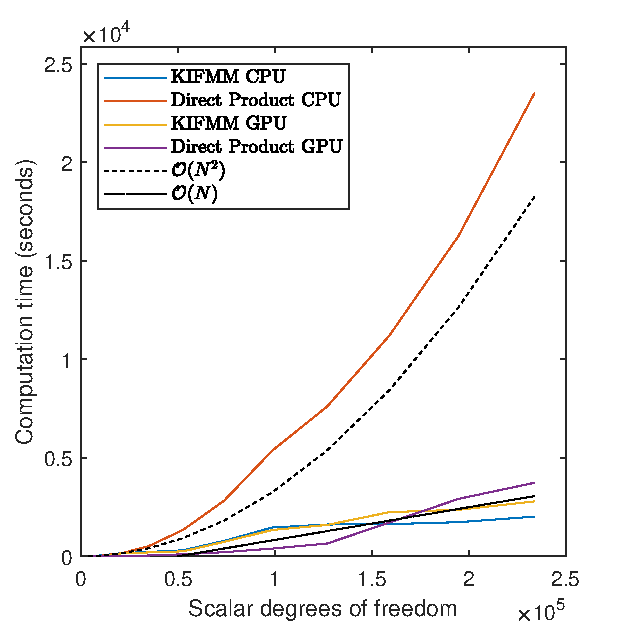
\includegraphics[width=\textwidth]{Images/KIFMM/Graphs/DirectProductCompTime.pdf}
         \caption{\label{fig:DirectProductCompTime}}
     \end{subfigure}
     \hfill
     \begin{subfigure}[b]{0.49\textwidth}
         \centering
         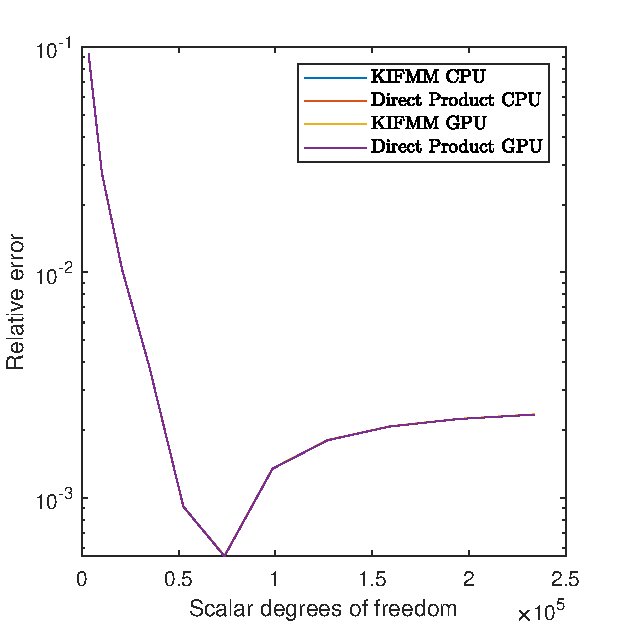
\includegraphics[width=\textwidth]{Images/KIFMM/Graphs/DirectProductComperror.pdf}
         \caption{\label{fig:DirectProductComperror}}
     \end{subfigure}
        \caption[Computation time and error for calculating the grand resistance matrix of a sphere using the KIFMM and Direct product methods.]{Computation time and error for calculating the grand resistance matrix of a sphere using the KIFMM and Direct product methods. (i) Computation time for computing the Grand Resistance matrix for a sphere at varying Scalar degrees of Freedom. (ii) The relative error in the computation of Grand Resistance error at various scalar degrees of freedom.}
        \label{fig:DirectProduct}
\end{figure}

Figure \ref{fig:DirectProductComperror} shows that all methods performed similarly when comparing their relative error from the exact solution. The increase in the error beyond $73000$ scalar degrees of freedom can be attributed to the regularisation error and quadrature error having opposite signs which cancel at this value. As the number of scalar degrees of freedom is increased the quadrature error continues to decrease and the total error approaches the regularisation error. More important is the error between the two solutions which maintained an absolute difference of less than $10^{-5}$ at all scalar degrees of freedom considered. Computation times differ more, with the CPU implementation of the direct product taking significantly longer than all other implementations. As expected, the direct product methods follow an order $N^2$ relation, with the GPU implementation growing much more slowly. The KIFMM methods grow by order $N$, with the CPU method outperforming our current GPU implementation. We would predict that this will continue to grow linearly for a given tolerance, as the number of GMRES iterations required to converge will grow slower than the number of scalar degrees of freedom. Understanding that the KIFMM method can perform the matrix-vector operations needed to solve the system in less time than the direct product, we will explore how changes to the KIFMM internal parameters affect this method's accuracy. 

\begin{figure}[ht]
     \centering
     \begin{subfigure}[b]{0.49\textwidth}
         \centering
         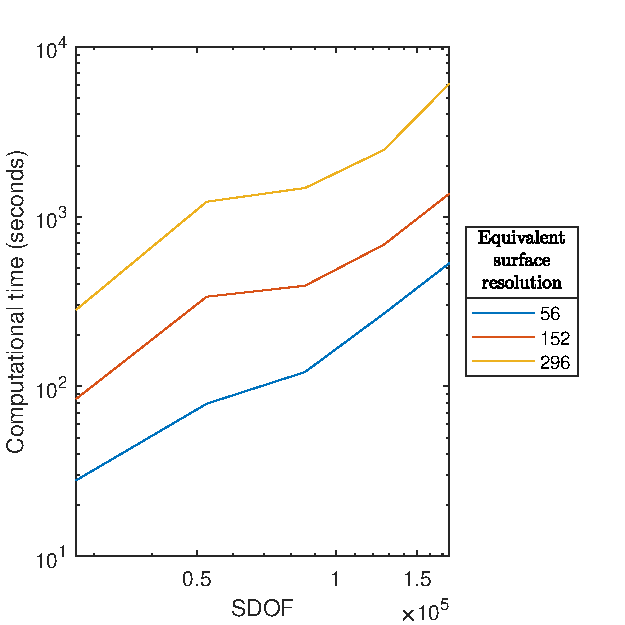
\includegraphics[width=\textwidth]{Images/KIFMM/Graphs/QuadPointsTime.pdf}
        \caption{\label{fig:QuadPointsTime}}
     \end{subfigure}
     \hfill
     \begin{subfigure}[b]{0.49\textwidth}
         \centering
         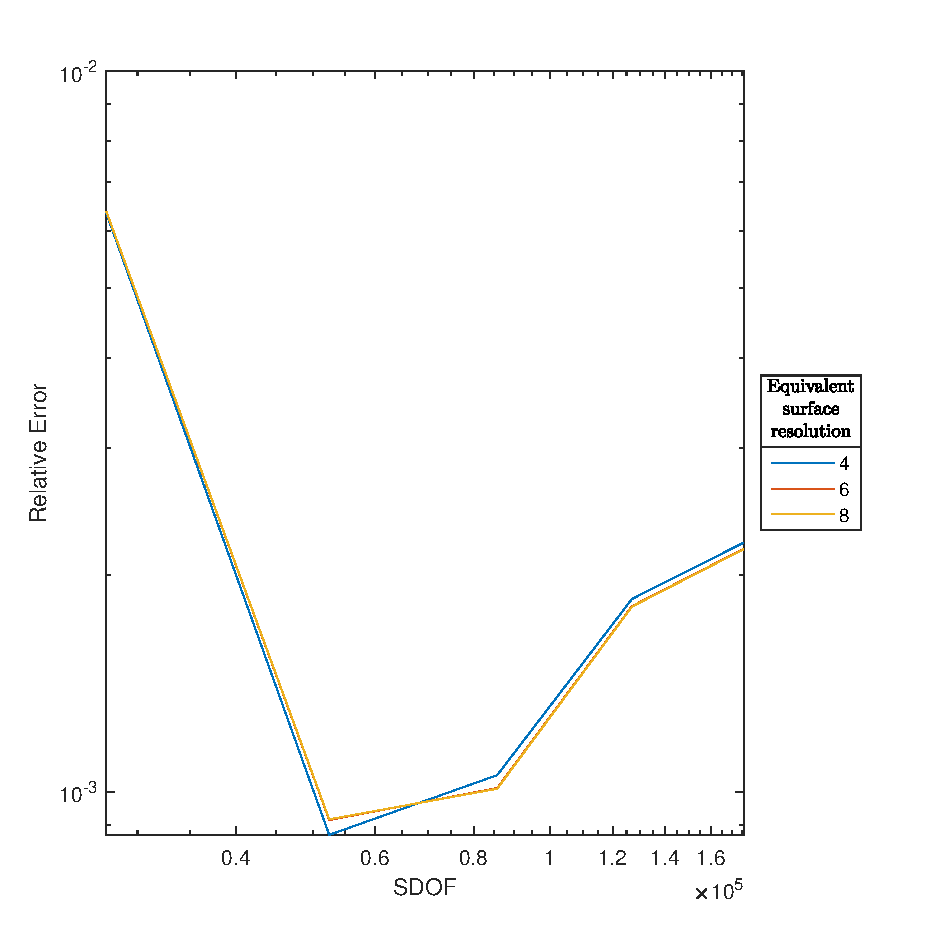
\includegraphics[width=\textwidth]{Images/KIFMM/Graphs/QuadPointsError.pdf}
         \caption{\label{fig:QuadPointsError}}
     \end{subfigure}
        \caption[Computation time and error for calculating the grand resistance matrix of a sphere using the KIFMM using $4\times4\times4$, $6\times6\times6$, $8\times8\times8$ Cartesian grids.]{Computation time and error for calculating the grand resistance matrix of a sphere using the KIFMM using $4\times4\times4$, $6\times6\times6$, $8\times8\times8$ Cartesian grids. (i) Computation time for computing the Grand Resistance matrix for a sphere at varying Scalar degrees of Freedom. (ii) The relative error in the computation of Grand Resistance error at various scalar degrees of freedom.}
        \label{fig:QuadPoints}
\end{figure}

As shown in \cref{fig:QuadPointsTime} the KIFMM becomes more costly when a finer mesh with more quadrature points is used to discretise the equivalent surfaces as the size of the linear systems which need to be solved increases. While the computation time of the problem increases, the error associated with the method decreases as the two integrals \cref{eq:upsurfint,eq:downsurfint} become more accurately approximated. For most simulations in this paper, a $6\times6\times6$ Cartesian grid was used for the equivalent surfaces as it provides accurate results with a reasonable computation time at all degrees of freedom we will consider. Note that if we had considered a finer quadrature based on a larger Cartesian grid the KIFMM method is still more efficient than the direct product for most scalar degrees of freedom, particularly when using CPU computation. 

The data in \cref{fig:NodeCap} was generated based on a fixed $6\times6\times6$ cartesian grid for the equivalent surface and the maximum node capacity changed when generating the Octree. All experiments show similar results for the error achieved, with smaller node capacities having fractionally better results as the initial equivalent surfaces form a better representation of the contained force points. In most cases, we see a trend where larger node capacities have shorter computation times as the overall Octree is smaller. This does mean more particle to particle interactions need to be considered which can slow the method down compared to methods with smaller node capacities. 

\begin{figure}[ht]
     \centering
     \begin{subfigure}[b]{0.49\textwidth}
         \centering
         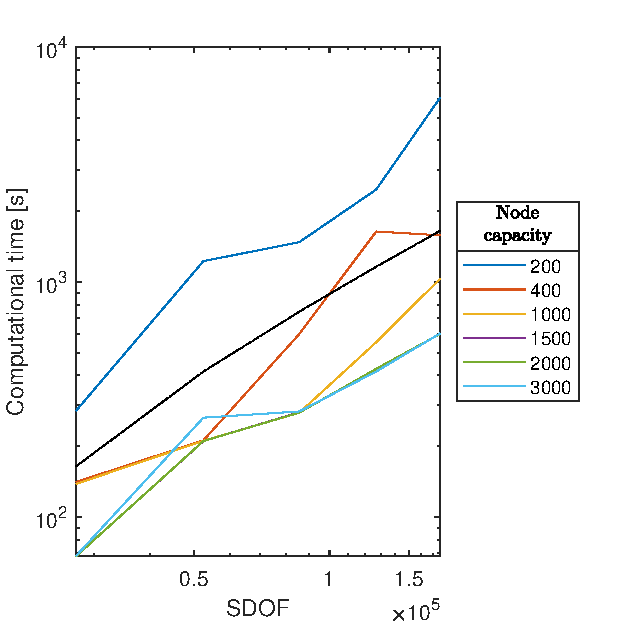
\includegraphics[width=\textwidth]{Images/KIFMM/Graphs/NodeCapTime.pdf}
         \caption{\label{fig:NodeCapTime}}
     \end{subfigure}
     \hfill
     \begin{subfigure}[b]{0.49\textwidth}
         \centering
         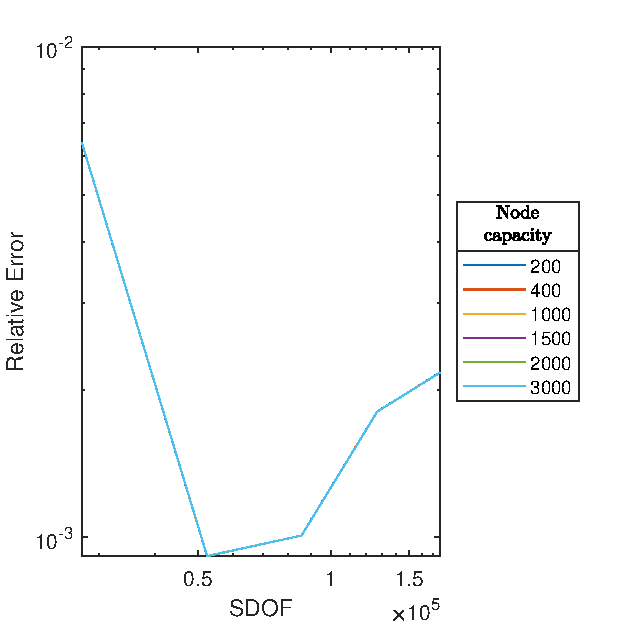
\includegraphics[width=\textwidth]{Images/KIFMM/Graphs/NodeCapError.pdf}
         \caption{\label{fig:NodeCapError}}
     \end{subfigure} \\
%     \begin{subfigure}[b]{0.49\textwidth}
%         \centering
%         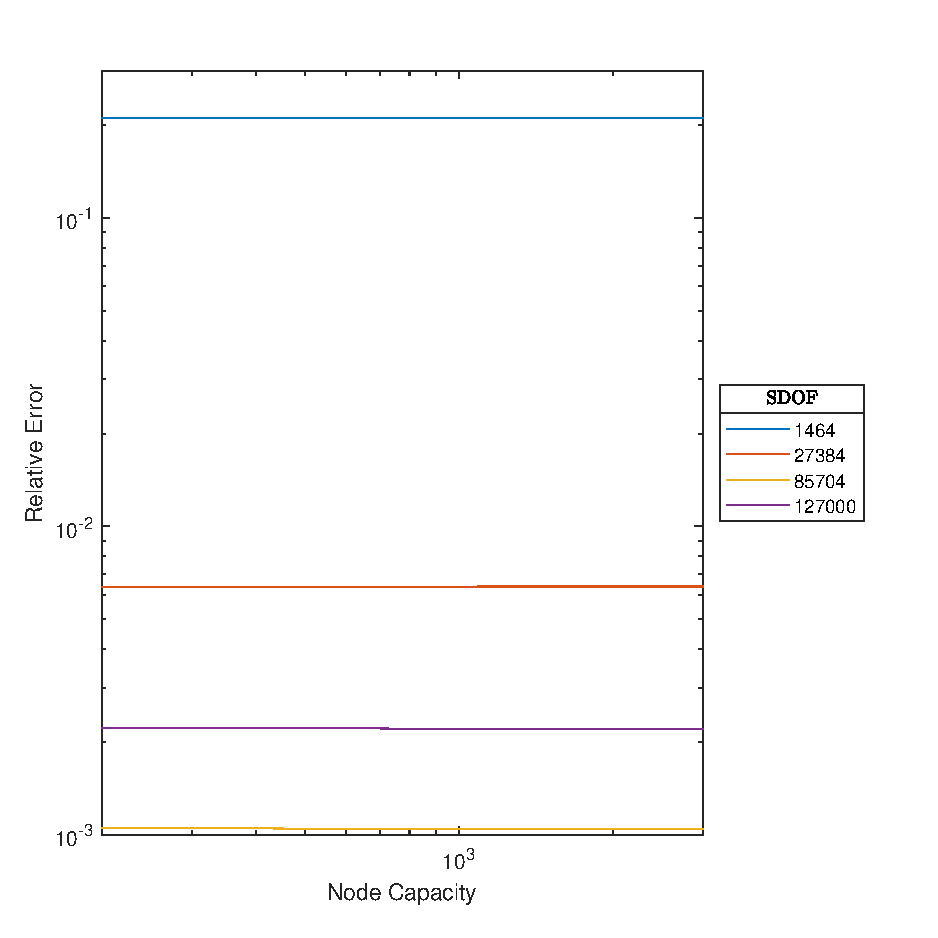
\includegraphics[width=\textwidth]{Images/KIFMM/Graphs/NodeCapError2.pdf}
%         \caption{Relative error in computation of Grand Resistance error at various scalar degrees of freedom}
%         \label{fig:NodeCapError2}
%     \end{subfigure}
        \caption[Computation time and error for calculating the grand resistance matrix of a sphere using the KIFMM and Direct product methods.]{Computation time and error for calculating the grand resistance matrix of a sphere using the KIFMM and Direct product methods. (i) Computation time for computing the Grand Resistance matrix for a sphere at varying Scalar degrees of Freedom. (ii) The relative error in the computation of Grand Resistance error at various scalar degrees of freedom.}
        \label{fig:NodeCap}
\end{figure}
